%%%%%%%%%%%%%%%%%%%%%%%%%%%%%%
\chapter{Conception}
%%%%%%%%%%%%%%%%%%%%%%%%%%%%%%

\section{Interface graphique}

Comme nous l'avons précisé précédemment, notre interface graphique se présente sous la forme d'un site Web. 

\begin{figure}[!ht]
	\begin{center}
		\fbox{
   		 \begin{minipage}[c]{0.9\textwidth}
  			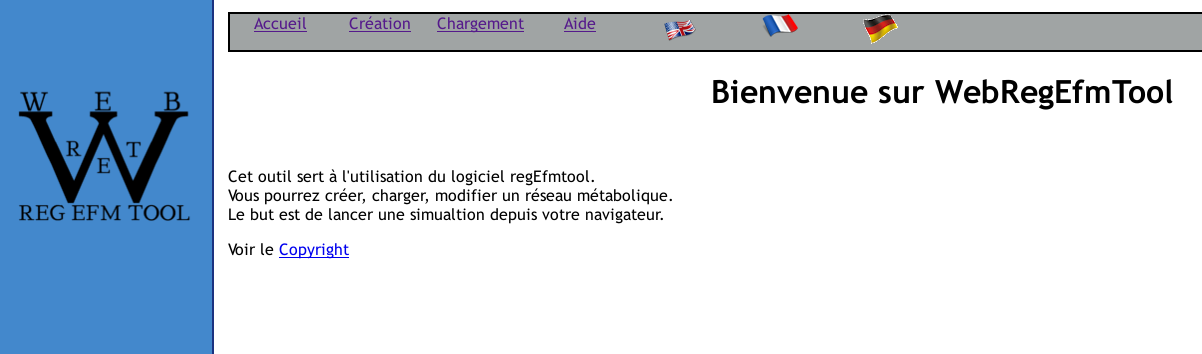
\includegraphics[width=0.90\textwidth]{../Images/Rapport/pageAccueil.png}  
		 \end{minipage}}
		\caption{Page d'accueil}
  		\label{main}
  	\end{center}	
\end{figure}

Lorsqu'un utilisateur arrive sur le site, une page d'accueil s'affiche (Figure \ref{main}). Elle contient des informations relatives à l'utilisation du programme (à quoi il sert, que peut-on y faire ...). A partir de là, deux choix s'offrent à lui:
\begin{itemize}
\item Soit il créé un nouveau réseau, en cliquant sur \emph{Création} dans le menu situé en haut de page,
\item Soit il charge un réseau qu'il a déjà créé en cliquant sur \emph{Chargement}.\\
\end{itemize}

Chaque page du site se présente de la m\^eme façon: un menu en haut de la page et le logo du site Web dans un bandeau situé sur la gauche.\\
Le menu contient quatre onglets:
\begin{itemize}
\item \emph{Accueil} qui permet de retourner sur la page d'accueil du site Web,
\item \emph{Création} qui permet de créer un nouveau réseau métabolique,
\item \emph{Chargement} qui permet de charger un réseau pré-existant,
\item \emph{Aide} qui permet de consulter une aide à l'utilisation du site.
\end{itemize}
On trouve aussi dans le menu, trois drapeaux qui permettent de changer la langue du site Web. Les trois langues proposées sont: l'anglais, le français et l'allemand. Par défaut le site est en français.

\section{Création d'un nouveau réseau}

Si l'utilisateur choisi de créer un nouveau réseau, il arrive sur une page qui va lui permettre d'ajouter de nouvelles réactions à celui-ci. \\

Une première partie permet d'initialiser les fichiers (Figure \ref{creation1}) dans le cas où l'utilisateur aurait déjà créé un réseau précédemment.\\

\begin{figure}[!ht]
	\begin{center}
		\fbox{
   		 \begin{minipage}[c]{0.9\textwidth}
  			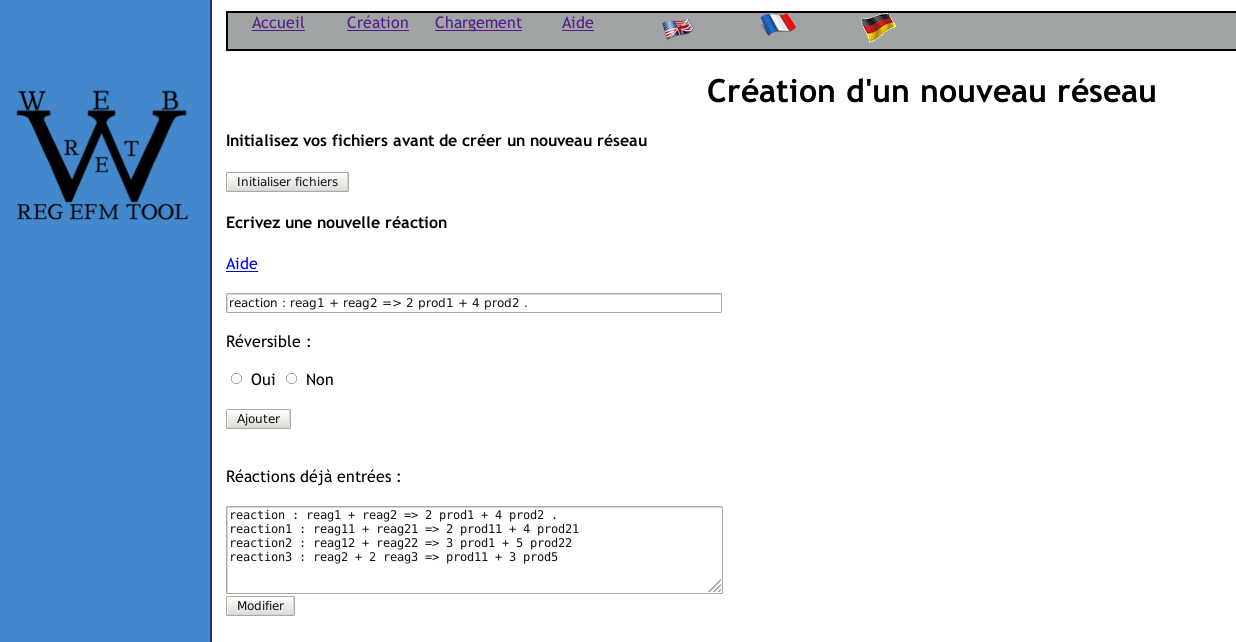
\includegraphics[width=0.90\textwidth]{../Images/Rapport/creation1.png}  
		 \end{minipage}}
		\caption{Page de création d'un nouveau réseau}
  		\label{creation1}
  	\end{center}	
\end{figure}

Une seconde partie permet de créer une nouvelle réaction. Celle-ci doit être de la forme $reaction : reag1 + reag2 => 2 prod1 + 4 prod2$. \\
L'utilisateur doit également préciser si la réaction est réversible ou non. Ensuite il clique sur le bouton \emph{Ajouter}, la réaction est alors ajoutée au réseau et apparaît dans la zone de texte située en-dessous. Dans cette zone de texte, l'utilisateur a la possibilité de modifier les réactions déjà créées (mais ne peut pas en ajouter ou en supprimer car les règles de réversibilités ne seraient alors pas respectées pour l'écriture d'un fichier au format \emph{.dat}). Il valide ensuite les modifications apportées en cliquant sur le bouton \emph{Modifier}.\\

\begin{figure}[!ht]
	\begin{center}
		\fbox{
   		 \begin{minipage}[c]{0.9\textwidth}
  			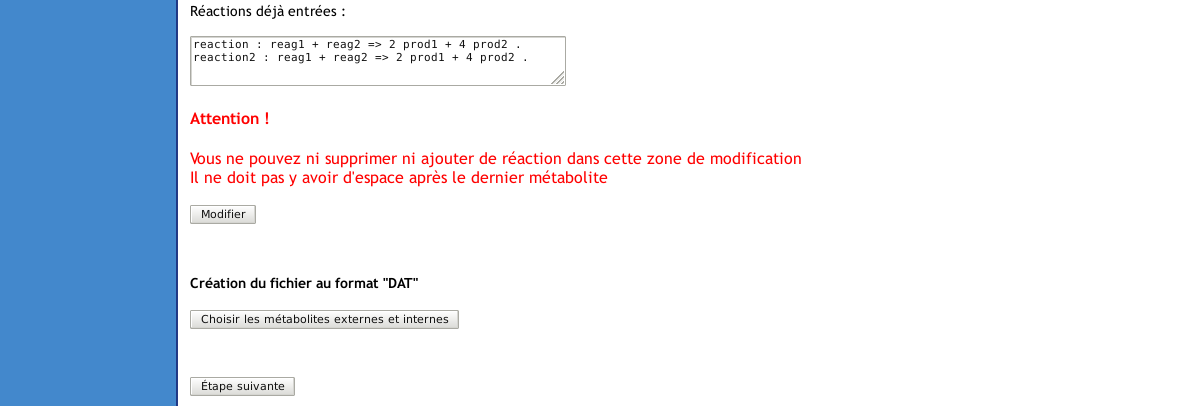
\includegraphics[width=0.90\textwidth]{../Images/Rapport/creation2.png}  
		 \end{minipage}}
		\caption{Suite de la page de création}
  		\label{creation2}
  	\end{center}	
\end{figure}

Enfin, l'utilisateur peut aussi générer un fichier au format \emph{.dat} (Figure \ref{creation2}) qui pourra être utilisé dans METATOOL par exemple.\\

\begin{figure}[!ht]
	\begin{center}
		\fbox{
   		 \begin{minipage}[c]{0.9\textwidth}
  			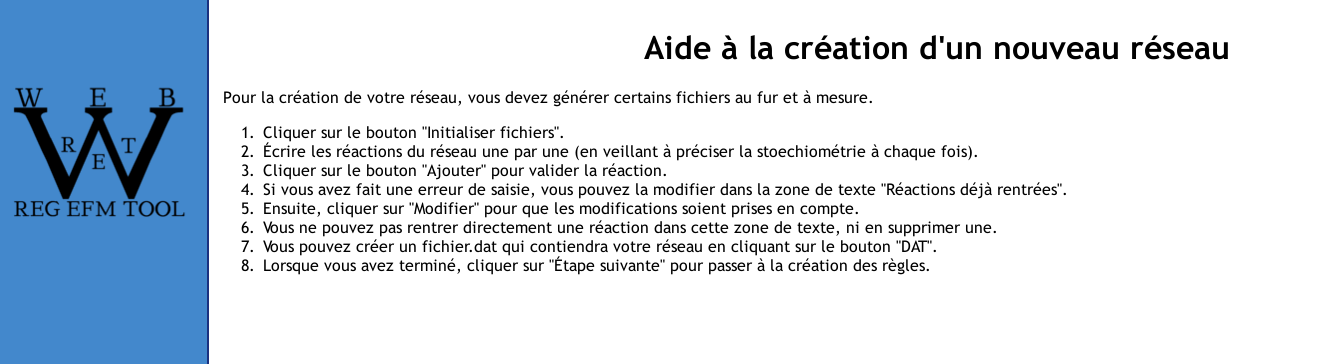
\includegraphics[width=0.90\textwidth]{../Images/Rapport/helpCreation.png}  
		 \end{minipage}}
		\caption{Page d'aide à la création d'un nouveau réseau}
  		\label{helpCreation}
  	\end{center}	
\end{figure}

Si l'utilisateur ne sait pas comment faire, il lui suffit de cliquer sur \textit{Aide} et une nouvelle fen\^etre de navigation (Figure \ref{helCreation}) appara\^itra afin de la guider. Cette page est automatiquement traduite dans la langue de la page courante. 

Quand l'utilisateur a fini de créer toutes les réactions qui composent son réseau, il clique sur le bouton \emph{\'Etape suivante} et arrive alors sur la page de création des règles des gènes.

\section{Règles des gènes}

Ces règles sont utilisées pour éliminer les modes élémentaires non possibles dans un réseau métabolique réel.\\

Une réaction R peut \^etre 1-active (R=1), 0-active (R=0) ou encore full-active (R=f).\\
La création des règles est régie selon certains principes:
\begin{itemize}
\item La réaction de sortie ne peut jamais être une réaction d'entrée. \\On ne peut pas écrire: R3 = ( ! ( ( ! 0R3) $|$  1R1) )
\item Une réaction peut être utilisée plusieurs fois comme réaction d'entrée. \\Ex: R11 = ( ( ! ( ( ! 0R3) $|$ 1R5) ) \& 1R3)
\item Le préfixe d'une réaction n'est valable que pour une opération.\\ Ainsi dans la règle R11 = ( ( ! ( ( ! 0R3) $|$ 1R5) ) \& 1R3), la réaction R3 est 0-active dans l'opération OR et 1-active dans l'opération AND.
\item Chaque réaction doit être entourée d'exactement une paire de parenthèses. \\R3 = ( ! 0R1 ) est correcte, mais R3 = ( ( ! 0R1) ) et R3 = ! 0R1 sont incorrectes
\item Il n'existe pas d'opération permettant de représenter la relation R2 = R1, elle sera représentée de la façon suivante: R2 = (fR1 $|$ fR1).\\
\end{itemize}

\begin{figure}[!ht]
	\begin{center}
		\fbox{
   		 \begin{minipage}[c]{0.9\textwidth}
  			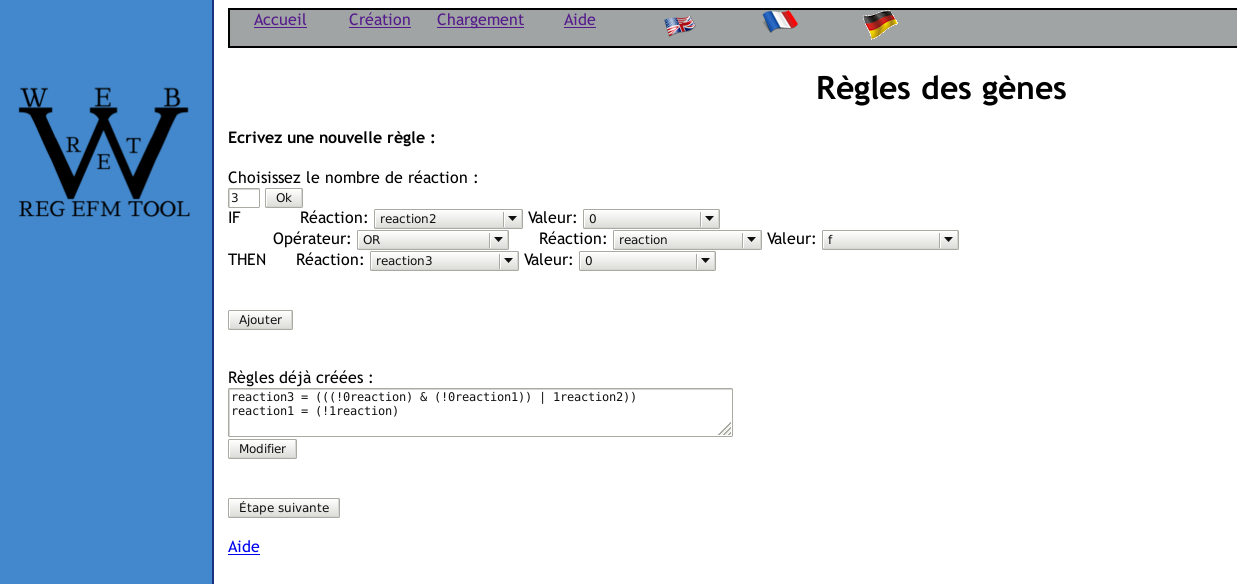
\includegraphics[width=0.90\textwidth]{../Images/Rapport/generules.png}  
		 \end{minipage}}
		\caption{Page de création des règles des gènes}
  		\label{generules}
  	\end{center}	
\end{figure}

Tout d'abord, l'utilisateur choisi le nombre de réactions qui composent la règle qu'il veut créer.
Une fois ce choix effectué, il clique sur le bouton \emph{Ok}. S'affichent alors de deux ou trois menus déroulant par réaction. Quand il y en a trois (Figure \ref{generules}), le premier permet de choisir l'opérateur, le second la réaction et le dernier sa valeur (0, 1 ou f). Quand il y en a deux, ils correspondent à la réaction et à sa valeur. L'utilisateur doit entrer un nombre de réactions au moins égal à deux.\\

L'utilisateur ne peut sélectionner le nom d'une réaction que lorsqu'il a choisi la précédente. Ceci permet de ne proposer que les réactions non sélectionnées précédemment pour le choix de la  réaction de sortie (principe utilisé dans la documentation de \emph{regEfmtool}).\\

Enfin, quand l'utilisateur a sélectionné toutes les réactions ainsi que leur valeur, il clique sur le bouton \emph{Ajouter}. La règle est alors écrite dans le fichier \emph{generules.grfile} si l'utilisateur a bien rempli tous les champs. Celle-ci apparaît alors dans la zone de texte située en-dessous. Dans cette zone, l'utilisateur a la possibilité de modifier, ajouter ou supprimer une règle déjà écrite, mais également d'en écrire de nouvelles manuellement. Lorsqu'il a fini ses modifications, il clique sur le bouton \emph{Modifier}, le fichier \emph{generules.grfile} est alors modifié en conséquence.\\

\begin{figure}[!ht]
	\begin{center}
		\fbox{
   		 \begin{minipage}[c]{0.9\textwidth}
  			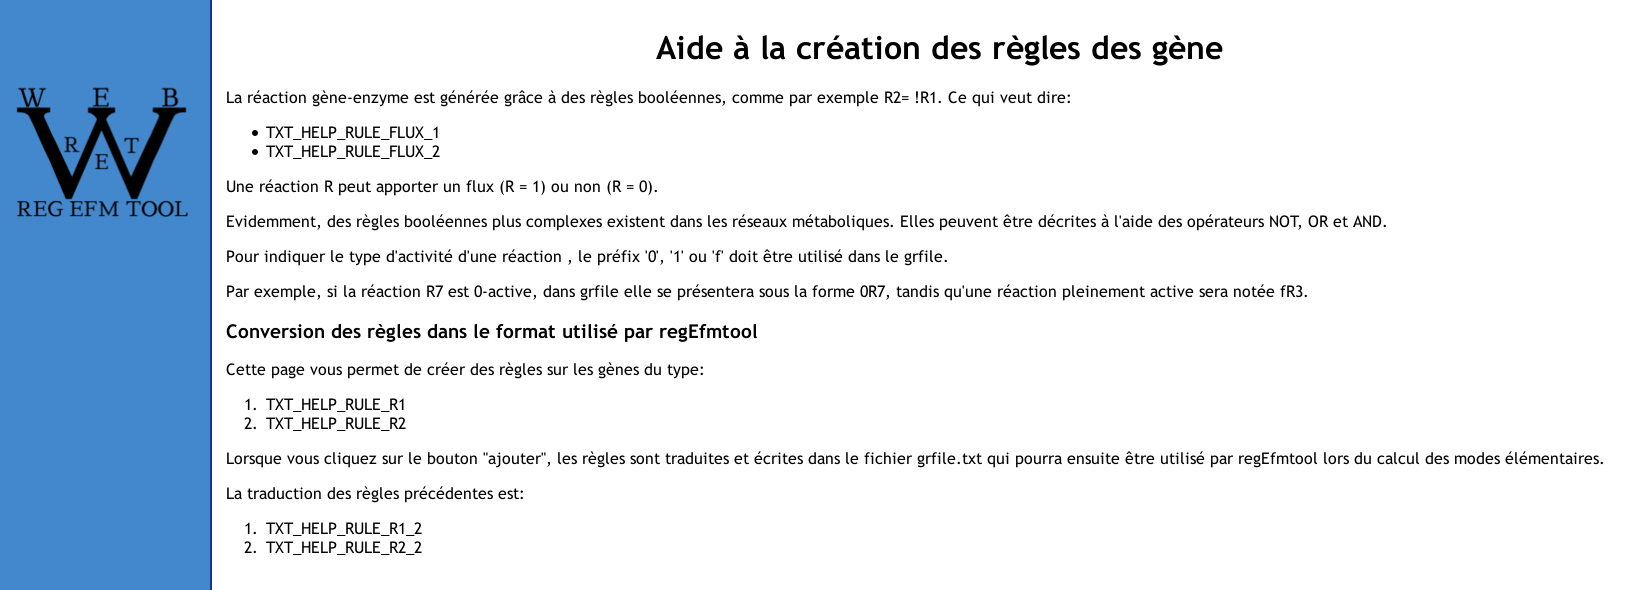
\includegraphics[width=0.90\textwidth]{../Images/Rapport/helpGenerules.png}  
		 \end{minipage}}
		\caption{Page d'aide à la création des règles des gènes}
  		\label{helpGenerules}
  	\end{center}	
\end{figure}

Si l'utilisateur ne sait pas comment faire, il lui suffit de cliquer sur \textit{Aide} comme précédemment et une nouvelle fen\^etre de navigation (Figure \ref{helpGenerules}) appara\^itra afin de la guider. Cette page est également automatiquement traduite dans la langue de la page courante. 

Une fois les règles entrées, l'utilisateur peut passer à l'étape suivante en cliquant sur le bouton correspondant. Il arrive alors sur la page de sélection des options nécessaires au lancement de la commande regEfmtool.

\section{Choix des options de lancement}

Comme nous l'avons dit précédemment, regEfmtool se lance gr\^ace à une ligne de commande. Cette page d'options (Figure \ref{options}) permet donc à l'utilisateur de sélectionner les paramètres de calcul qu'il souhaite, par la biais de boutons à cocher. Certaines options sont pré-cochées, se sont les options de base nécessaires au bon déroulement des calculs du logiciel. Cela permet à un utilisateur non expérimenté de lancer ses calculs avec le réseau qu'il vient de créer. Un utilisateur plus averti pourra modifier ces options à sa guise afin d'avoir un niveau de complexité d'exécution des calculs supérieur.\\

\begin{figure}[!ht]
	\begin{center}
		\fbox{
   		 \begin{minipage}[c]{0.9\textwidth}
  			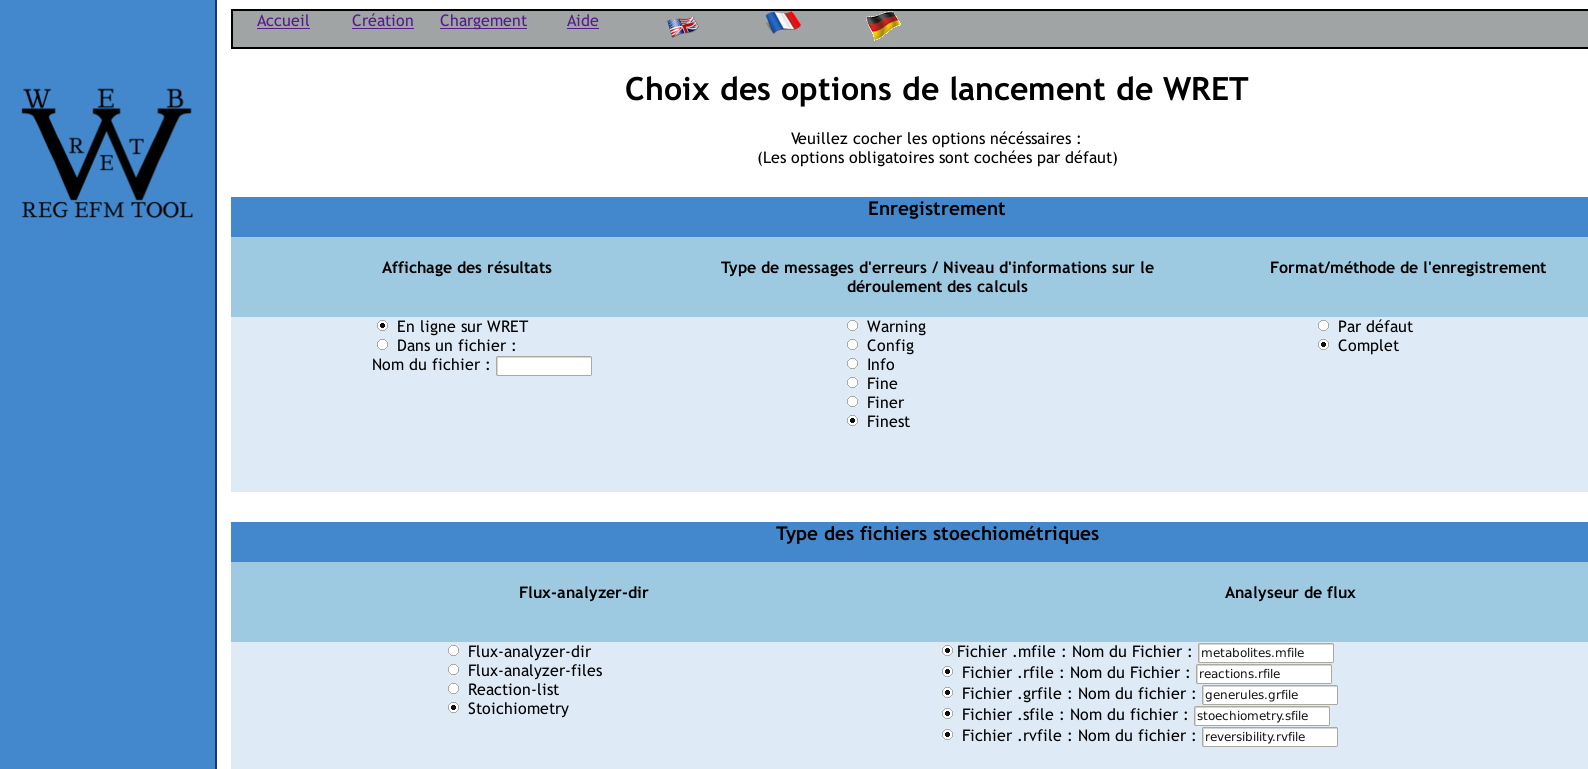
\includegraphics[width=0.90\textwidth]{../Images/Rapport/options.png}  
		 \end{minipage}}
		\caption{Partie de la page de choix des options de lancement}
  		\label{options}
  	\end{center}	
\end{figure}

Les options sont regroupées par catégories (en fonction de ce qui était précisé dans le fichier \textit{metabolic-efm.xml} de regEfmtool):

\paragraph*{Enregistrement} Cette catégorie contient trois sous catégories précisant le type d'affichage des résultats, le niveau d'informations sur le déroulement des calculs et le format d'enregistrement. Par défaut, l'affichage se fera en ligne sur le site et le type de message d'information est le plus complet possible. 

\paragraph*{Types de fichiers stœchiométriques} Cette catégorie possède deux sous catégories précisant le type de parsage en entrée et l'analyseur de flux. Cette dernière permet de définir les types de fichiers d'entrée que regEfmtool utilisera. Ces fichiers étant lors des étapes précédentes, leurs noms sont déjà pré-rentrés dans les cases correspondantes.

\paragraph*{Compression et paramètres de sortie} Ces deux catégories contiennent chacune une seule sous catégorie, servant respectivement à définir le niveau de compression (et également l'utilisation de la récursivité dans les calculs) et le type de fichier désiré en paramètre de sortie. L'option "text-doubles" est cochée par défaut, avec le nom du fichier qui contiendra les modes élémentaires calculés. Nous avons appelé ce fichier \textit{results.txt}. 

\paragraph*{Paramètres d'Efmtool} Cette dernière catégorie contient sept sous catégories: le "\textit{rowordering}" (ou la ligne de commande à utiliser), la méthode d'adjacence, le nombre maxiamal de "\textit{threads}" (prédéfini à 2 suivant les exemples de regEfmtool), l'arithmétique des nombres, le type de normalisation pour la sortie (prédéfinie à "aucune"), la précision fractionnaire et l'activation ou non d'un auto-test après chaque itération. \\

Une fois que l'utilisateur a coché toutes les options qu'il souhaite, il lui suffit de cliquer sur le bouton \emph{Lancement} afin de générer la commande et lancer regEfmtool. Ensuite, une page d'affichage des résultats s'affiche. 

\section{Chargement d'un réseau pré-existant}

Cette page accessible depuis le menu général permet à un utilisateur de charger un réseau préexistant depuis son disque dur. Il pourra également générer la ligne de commandes nécessaire au lancement de regEfmtool. Cette page est basée sur le modèle de la page du choix des options, à un détail près : dans la catégorie du type des fichiers stœchiométriques, les fichiers ne sont pas prédéfinis mais c'est à l'utilisateur à les charger. Le reste fonctionne de la m\^eme façon que précédemment. Les noms de fichiers (et leurs chemins relatifs) sont récupérés et la ligne de commande est créée. \\

\begin{figure}[!ht]
	\begin{center}
		\fbox{
   		 \begin{minipage}[c]{0.9\textwidth}
  			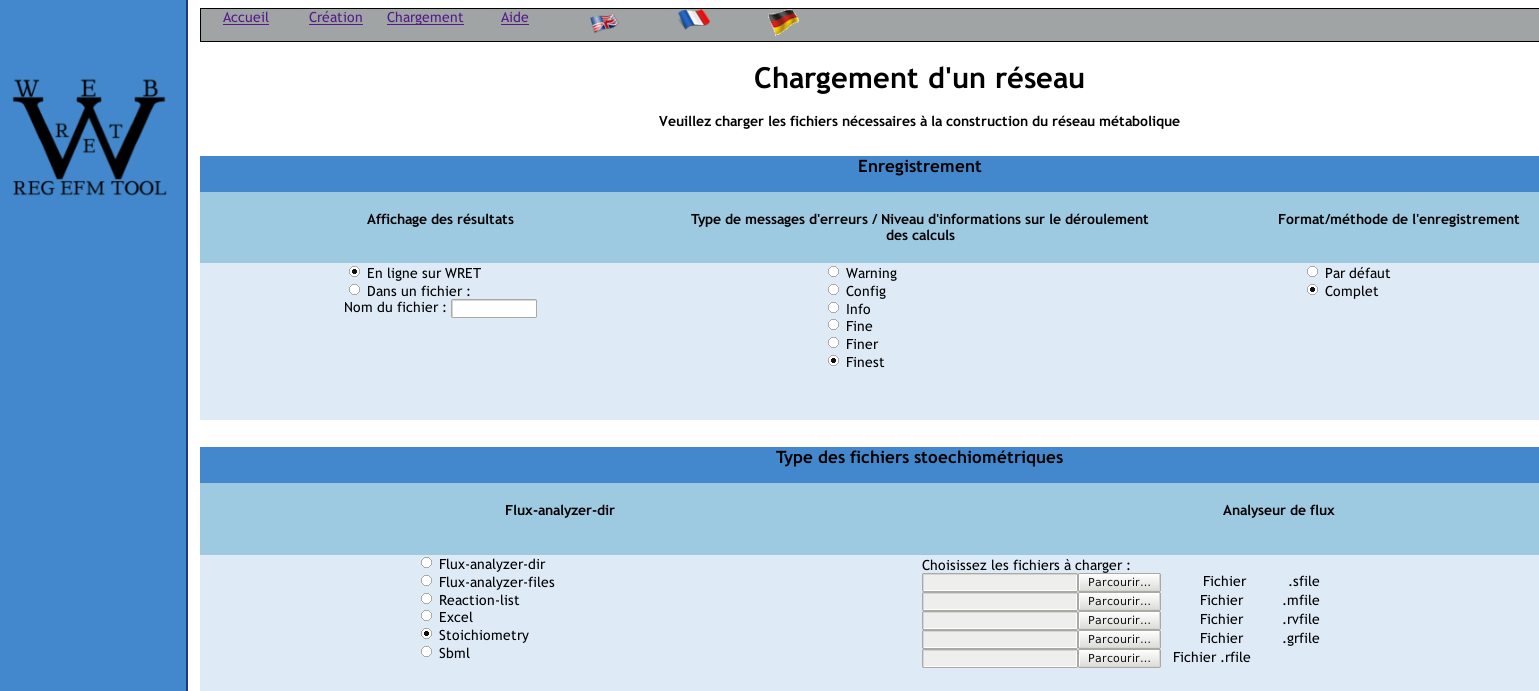
\includegraphics[width=0.90\textwidth]{../Images/Rapport/chargement.png}  
		 \end{minipage}}
		\caption{Partie de la page de chargement d'un réseau préexistant}
  		\label{chargement}
  	\end{center}	
\end{figure}

L'utilisateur n'aura plus qu'à cliquer sur \textit{Lancement} pour lancer la récupération des noms des fichiers (et leurs chemins relatifs) ainsi que la création de la ligne de commande et le démarrage du logiciel. Une page de résultats s'affichera ensuite. 

\section{Affichage des résultats}















 